\clearpage

A LaTex nyelv elsajátítása, irodalomkutatás, valamint a dokomentum írása megközelítőleg két és fél hetet vett igénybe, az ezutáni néhány napban, pedig a konzultációk utáni kisebb változtatások,javallatok, kérések eszközlésével foglalkoztam, majd véglegesnek minősítettük az eredményt.

\subsection *{Prezentációt segítő anyagok}

A gyakorlat második felében a cél olyan később is felhasználható anyagok készítése volt, amik a kvantumkommunikáció, valamint annak mára már egyre növekvő ipari jelenlétének bemutatására használhatóak. Kiindulópontnak egy a kvantumkommunikáció fejlődését bemutató timeline, valamint egy a jelenlegi kvantumkommunikációs ipari helyzetet leíró térképet határoztunk meg célnak.\\ 
A munkámat a timeline elkészítésével kezdtem, mivel az ide gyűjtendő információkból rendelkeztem egy kevés előismerettel. Ennek következtében arról is volt egy pontosabb elképzelésem, hogy mi kerülhet majd a végtermékre. Az elkészüléshez szükséges idő nagy részét ebben az esetben is az irodalomkutatás vette el.  Véleményem szerint ez a kvantumos technológiák fiatalságának, valamint, annak, hogy ezen belül is a viszgálandó terület igen specifikus és szük volt. Ennek következtében a felhasználható források maguk is igencsak szűkösek voltak. A kezdeti évekhez hasznos forrásnak bizonyultak az akkoriban publikált témába vágó kutatások. Ezeknak a hátránya volt viszon, hogy bennük egy specifikus információ keresése igen nehézkes, sok esetben szükséges hozzá az egész dokumentum elolvasása.Ezekhez a részekhez azt a stratégiát alkalmaztam, hogy néhány jól megválasztott kulcsszóval a szűkebb témát ki tudtam szűrni a találatok közül(Google Scholar), majd a keresési idősáv egy évre történő leszűkítésével megkaptam az éppen aktuális évhez tartozó elolvasandó publikációkat. Ezen felül használtam még az olvasott publikációkban található hivatkozásokat is, hogy megtaláljam azt, ami fölött a fenti módszerrel esetlegesen átsiklanék. Az időben  későbbi adatok nagyrésze már nem feltétlen tudományos lapokban publikált kutatási eredmény volt, hanem a területen alakuló ipar eredményei. Itt az előző taktikát értelemszerűen már nem lehetett használni. Az említett adatok túlnyomóan cikkekből, azokban található hivatkozásokból származnak. A kész ábrával kapcsolatban elvárás volt, hogy vektorgrafikus legyen, ezért a Microsoft Visio program segítségével készítettem.\\
Az elkszült ábra.
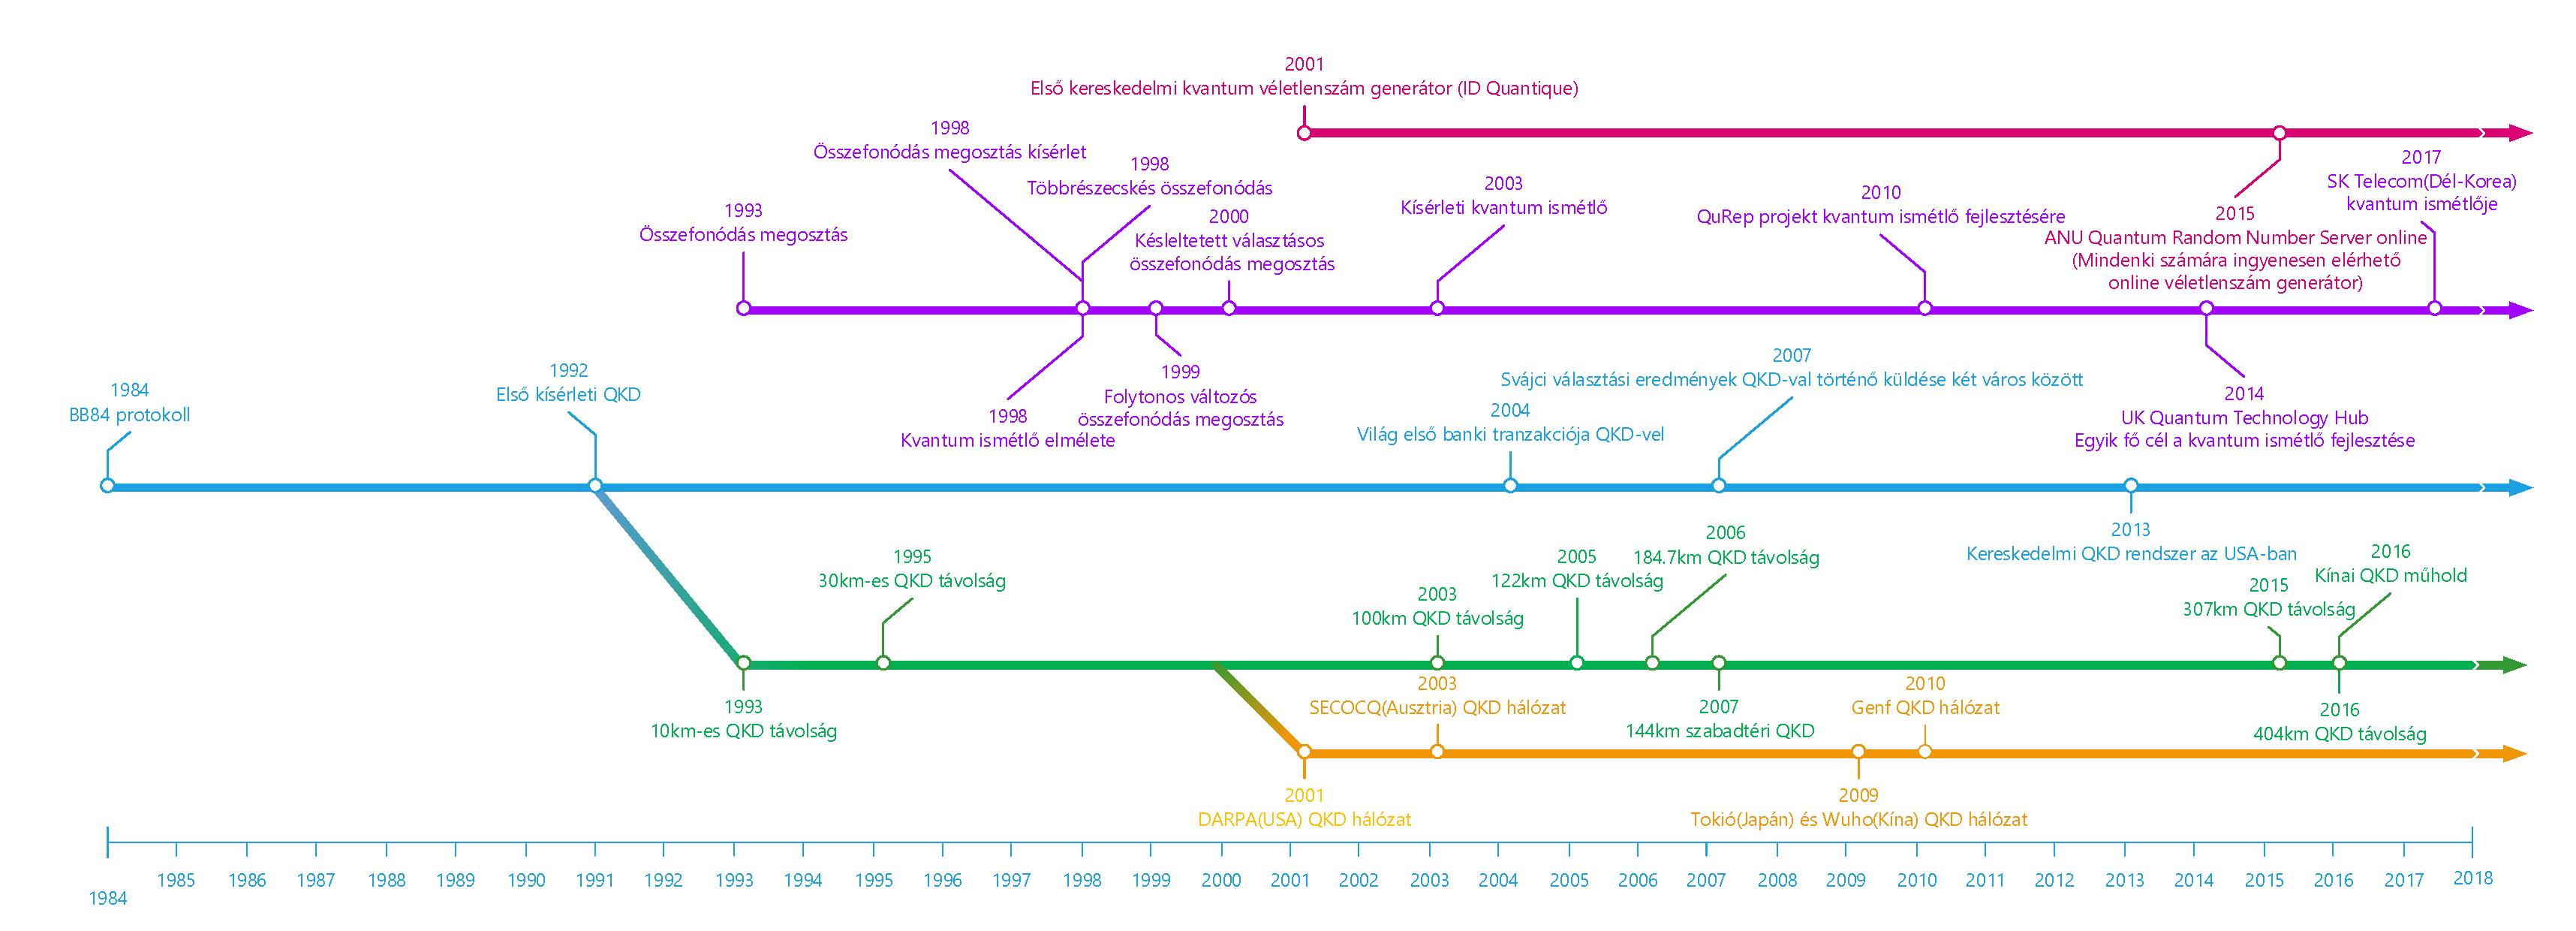
\includepdf{timeline}
A második feladatban kezdetben a cél egy világtérkép elkészítése volt az ipari szereplők feltüntetésére, amin a kvantumkommunikációs fejlesztéshez kapott támogatás/képviselt érték szerint lehetett volna színezni. Ezen sajnos a rendelkezére álló információk hiánya miatt részben változtatni kellet. Ennek megfelelően az ehhez tartozó irodalomkutatás jelentősebb része ennek kiderítésével telt. Itt nagyban mutatkozott a terület fiatalsága, valamint az ebből származó hátrányok a gyűjtés szempontjából. A legtöbb kizárólag témakörrel foglalkozó ipari szereplőről még nem találhatóak felmérések, cikkek. A nagyobb piaci szereplőkről pedig akik a témában kutatnak kisebb, nagyobb csoportokkal, részlegekkel, a technológiát hasznosító késztermék hiányában nincs olyan gazdasági említés, amiben ez a kis részleg/csoport kezelhető számokkal külön említésre kerülne.Használható kimutatást a témához összesen egyet találtam, körülbelül 1500 dollárért, emiatt a későbbi konzultáció után úgy döntöttünk, hogy a feladatott módosítjuk. Az új elkészítendő térkép ezek alapján bejegyzett kvantumkommunikációs cégekkel rendelkező országok szemléltetésére szolgál. Ehhez az előzővel ellentétben, habár még mindig nehézkesen, de már lehetett elégséges mennyiségű információt találni. Ehhez az ábrához is természetesen elvárás volt a vektorgrafikusság. Az összegyűjtött anyagok és az Adobe Illustrator program segítségével készült el végül az alábbi ábra:\\
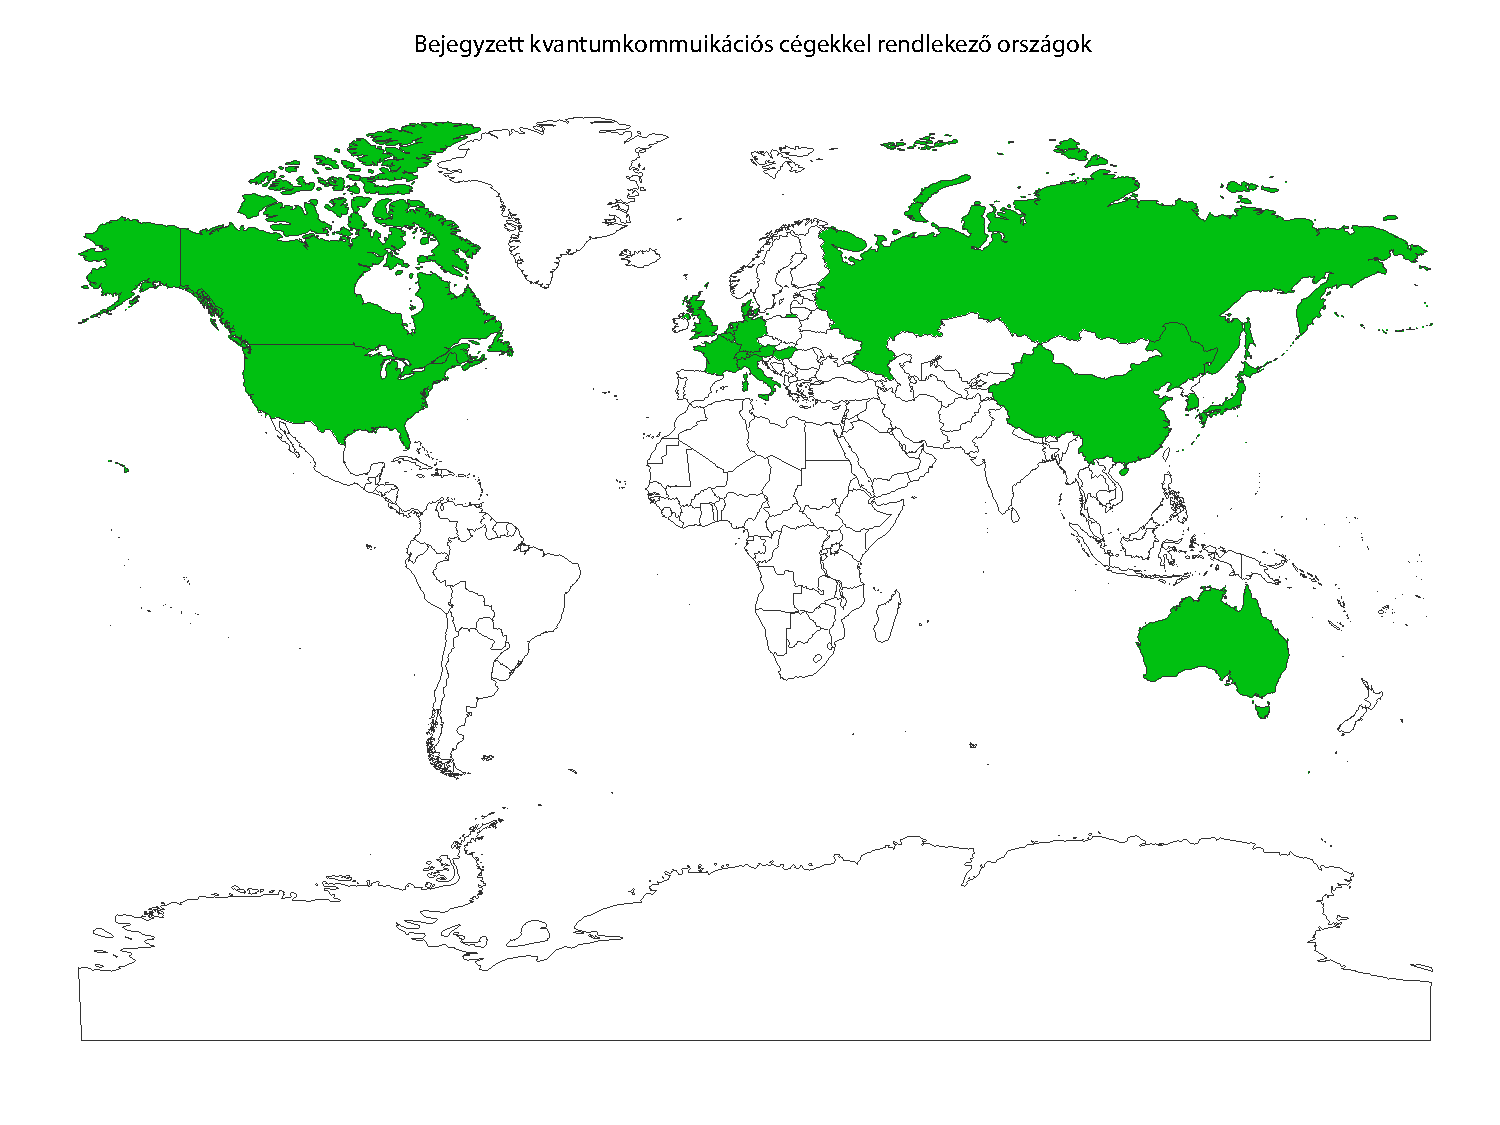
\includepdf{terkep}
Ezek után egy lehetséges plakát tervén kezdtem el dolgozni. Ennek témául a kvantumkommunikáció mint terület, valamint a kvantumismétlők, mint itteni előrelépési lehetőség rövid bemutatását tűztük ki célul. Ehhez a fentieken túl szükséges volt még néhány magyarázó ábra elkészítése, valamint a plakátra kerülendő szöveg megírása. Design tapasztalattal sajnos nem rendelkeztem,  kezdetben az így megalkotott anyagokból (timeline, térkép, ábrák, szöveg) próbáltam az Illustrator segítségével elfogadható plakátot varázsolni. Ekkorra már közeledett a gyakorlat vége, egy plakáttervvel el is készültem, viszont tudván, hogy megfelelő tapasztalattal szebbet és jobbat tudnék, megkérdeztem a konzulensem arról a lehetőségről, hogy a gyakorlat végeztével felkeresem egy ilyen témában jártasabb ismerősöm segítségért a plakát kinézetéhez. Ő készítette a következő tervet:\\
\includepdf{project}
A plakáton látható ábrák, valamint szövegek a gyakorlatom végének termékei, az elrendezés és design már a tapasztaltabb ismerősöm érdeme. A cím értelemszerűen placeholder szerepet tölt be. A design véglegeítését valószínüleg szeptember hónapban tudom befejezni, mivel ekkorra tudtunk csak találkozót megbeszélni az ismerősömmel aki a megjelenéstervet készítette.(Ez szükséges, mivel az általa a tervezéshez használt eszközöket én magam nem ismerem kellően) A tervet azóta a gyakorlatom rendezői is koncepciójában elfogadták, a talákozón már csak véglegesítés és rövid közös kidolgozás várható. Emiatt a most ismertetett koncepció a plakát végleges kinézetét, valamint elrendezését tekintve mérvadónak tekinthető.\\
\section*{Összefoglalás}
A gyakorlat során sok olyan tudást szereztem amit egyetemi tanulmányaim során eddig nem, egy már korábban tanulmányozott témát közelíthetttem meg egy új szemszögből. Az elvégzett feladatok, valamint az ezek során fellépő nehézségek rávilágítottak számomra arra, hogy egy-egy téma, munka, technológia elérhetősége mennyire sokat is számít, valamint, hogy ennek hiánya mekkora hátrányt jelenthet számára.

